%In this section we show that PAT leads to better transliteration models even without parallel data.
%
%\subsection{Generative Story}


%\subsection{Parameter Agreement Training}
%In PAT, the model corresponding to the inverse generative story is also used.
%This inverse process is illustrated at the bottom of Figure \ref{fig:fsts}.
%
%The training data for the reverse direction consists of set of English pronunciations  $E=\{\mathbf{e_n}\}_{n=1}^{|E|}$ and independent training maximizes:
%\begin{align}
%L(E)& = \sum_{\mathbf{e}\in E} \log \sum_{\mathbf{j}} \QQ(\mathbf{e}\mid \mathbf{j})\cdot \QQ(j)
%\end{align}
%To apply PAT, we maximize the joint regularized objective function:
%\begin{align}
%L(J) + L(E) + \lambda R(\PP(\mathbf{j}|\mathbf{e}), \QQ(\mathbf{e}|\mathbf{j}))
%\label{eqn:dec_obj}
%\end{align}
%Once the two models are trained, Japanese words can be decoded using either model. 
%In practice we followed Ravi and Knight and used the $\PP$.
%\begin{figure*}[t]
%\begin{center}
%\begin{tabular}{ccc}
% &  & \tabularnewline
% & 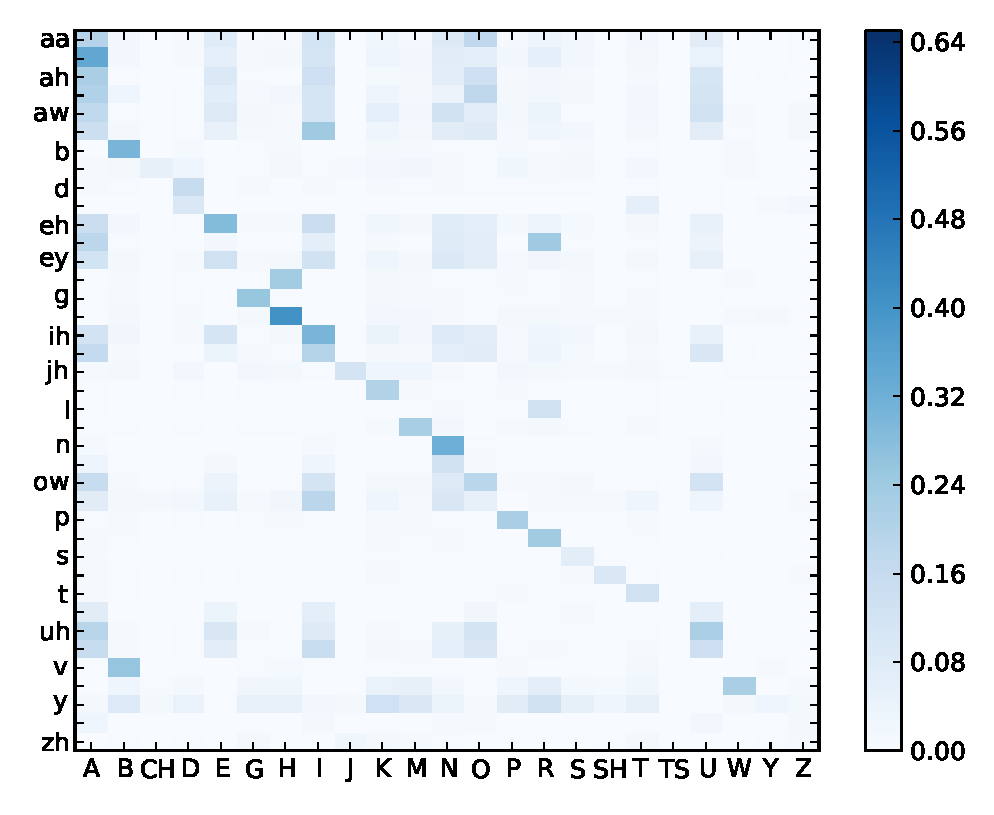
\includegraphics[scale=0.4]{figures/model_11_vanilla} &
% \includegraphics[scale=0.4]{figures/model_11_gm}\tabularnewline
% &  & \tabularnewline
%\end{tabular}
%\caption{Compared to independent training. PAT (right) learns sparser, peaked models.}
%\label{fig:mapping}
%\end{center}
%\end{figure*}

In this section we report our experiments on deciphering transliterations.
To compare our method PAT against independent training, we first reproduced the English-to-Japanese transliteration pipeline of \newcite{RK09} (as described in our section ? and depicted at the top of figure \ref{fig:fsts}) and tried to match their reported results (Unfortunately we were unable to obtain all their FSTs and data). We then constructed the inverse pipeline, required by our method PAT.

\subsection{The baseline decipherment model}
To reproduce the English-to-Japanese pipeline, we constructed the following FST models:
\begin{enumerate}
\item A unigram language model of English terms, estimated over the top 40K most frequent capitalized words found in the gigaword corpus (no smoothing was applied).
\item An English pronunciation FST from the CMU pronunciation dictionary (REFERENCE).
\item A English-to-Japanese phoneme mapping FST that encodes the phoneme transliteration table $t_1$ (see \eqn{eqn:trans}), constructed based on the best setting reported by \newcite{RK09}. 
We note that $t_1$ is restricted to either 1-to-1 or 1-to-2 phoneme mappings, maintaining consonant parity. See further details in their paper.
\item A hand-built Japanese pronunciation FST, provided by Kevin Knight.
\end{enumerate}

\newcite{RK09} report back-transliteration whole-name error rates (WNER) on a list of 100 transliterated US senator names (In WNER, a decoding is correct if both the first and last name are decoded correctly).
Using limited amounts of parallel data they report a 40\% WNER in the
parallel setting, compared to 73\% WNER on their best decipherment setting.

\subsection{The inverse model}
On top of the English-to-Japanese pipeline, implementing PAT requires a pipeline in the inverse direction - a Japanese-to-English transliteration pipeline (as depicted at the bottom of figure \ref{fig:fsts}), with similar FST models. 

We constructed a unigram language model of Katakana terms over the top 25K most frequent Katakana words found in the Japanese news 2005-2008 Leipzig corpora (REFERENCE).
%(http://corpora.informatik.uni-leipzig.de/download.html)

The remaining required FSTs were obtained by inverting the baseline FSTs (that is, FSTs 2,3,4). in particular, the Japanese-to-English phoneme mapping FST $t_2$ was obtained by inverting $t_1$.


\subsection{Training}
For training data we take the top 50\% most frequent terms in their respective language models.
Using the entire set of terms led to poor baseline results, possibly since uncommon English terms are not transliterated, and uncommon Katakana terms may be borrowed from languages other than English.
In any case, it is important to note that the two resulting sets of words are far from being parallel, since they were collected over non-parallel corpora.

EM training of the baseline pipeline was done using the Carmel finite-state toolkit (REFERENCE). 
The LM and pronunciation models were held fixed while the parameters of the phoneme mapping model $t_1$ were optimized to maximize likelihood of the observed set of Japanese terms.

Similarly the PAT objective (\eqn{eqn:joint}) was maximized with respect to the phoneme mapping models $(\TA, \TB) = (t_1, t_2)$, with coefficient $\lambda\in\{1,2,3,4\}$ and all other FSTs fixed (note that $\lambda=0$ corresponds to independent training, i.e. the baseline).
We manipulated Carmel to compute a single E-step and output the expected counts which we then used to formulate the M-step objective. The M-step was solved using our own projected gradient descent implementation (A python implementation of a general purpose PGD solver for convex functions over convex closed sets. to be released).

Training was limited to 15 EM iterations.

\subsection{Results}
We compiled a list of 100 US statesmen names (first and last) to be used as a test set. 
To tune $\lambda$ we used a development set consisting of 50 frequent Japanese terms and their English origin.

For each method, we selected the $t_1$ model that minimized the development back-transliteration error rate over the 15 iterations, $\lambda$ and the so-called stretch-factor 
$\alpha \in \{1,2,3\}$ that exponentiated the model parameters before decoding (see \cite{RK09}).
back-transliterations were obtained using Viterbi decoding.

Table \ref{tbl:transliteration_results} reports WNER, average normalized edit distance (NED) and the number of $t_1$ parameters with value greater than 0.01 ($t_1>0.01$) as an indication of model sparsity.

\begin{table}[h]
\begin{center}
\begin{tabular}{|c|c|c|c|}
\cline{2-4} 
\multicolumn{1}{c|}{} & WNER & NED & $t_1> 0.01$\tabularnewline
\hline 
Independent & 67\% & 23.18 & 649\tabularnewline
\hline 
PAT (our) & 59\% & 17.35 & 421\tabularnewline
\hline 
Parallel Data & 43\% & 10.8 & 152\tabularnewline
\hline 
\end{tabular}
\label{tbl:transliteration_results}
\caption{PAT reduces error rates and learns sparser models.}
\end{center}
\end{table}

Figure \ref{fig:mapping} compares a portion of the best phoneme mapping table learned by the baseline and PAT, showing a difference in parameter sparsity.
\begin{figure*}[t]
\begin{center}
\begin{tabular}{ccc}
 &  & \tabularnewline
 & 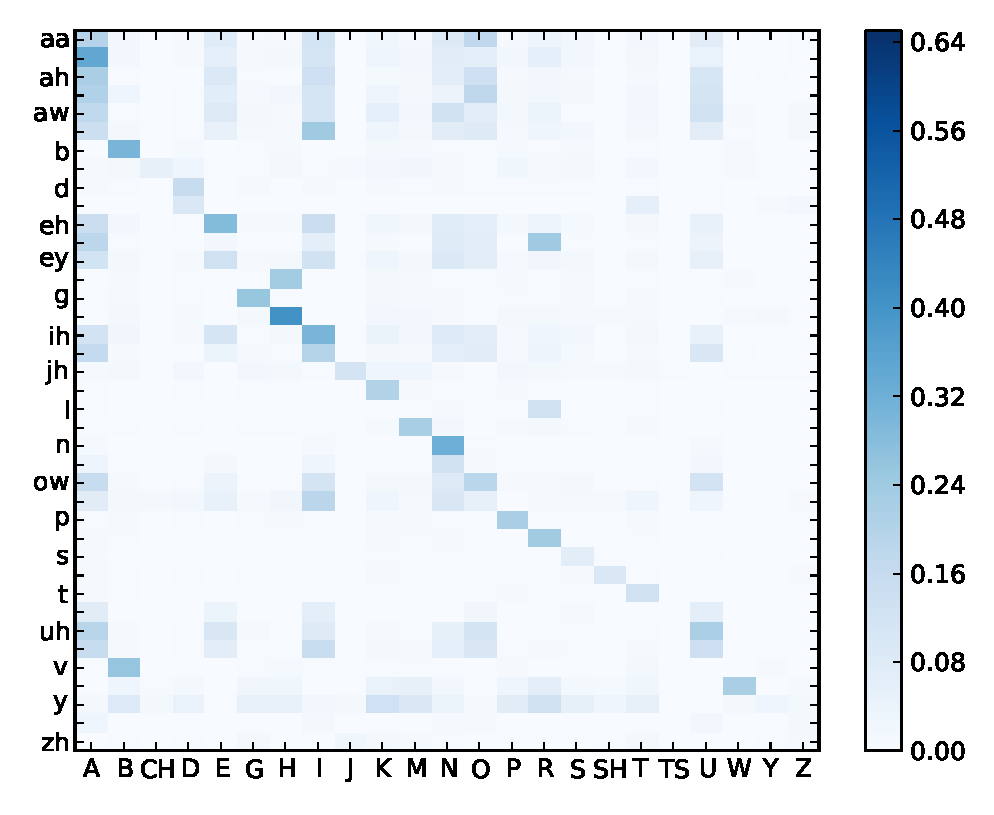
\includegraphics[scale=0.4]{figures/model_11_vanilla} &
 \includegraphics[scale=0.4]{figures/model_11_gm}\tabularnewline
 &  & \tabularnewline
\end{tabular}
\caption{Compared to independent training. PAT (right) learns sparser, peaked models.}
\label{fig:mapping}
\end{center}
\end{figure*}





%
%\subsection{Decipherment Experiments}
%In this section we report our experiments on deciphering transliterations.
%Ravi and Knight \cite{RK09} compare back-transliteration whole-name error rates (WNER) on a list of 100 US senator names (In WNER, a decoding is correct if both the first and last name are decoded correctly).
%They report 40\% error rate in the
%parallel setting, and a 73\% error rate when using their best decipherment setting.
%
%In order to compare PAT against independent training, we reproduced the decipherment setting \cite{RK09}.
%For the FST machinery, we prepared:
%\begin{itemize}
%\item An English pronunciation FST from the CMU pronunciation dictionary. A Japanese pronunciation FST that was hand built.
%\item Pronounceable word unigram LMs, constructed over the top ~40K most frequent capitalized words in the gigaword corpus and the top ~25K most frequent Katakana terms in the Japanese news 2005-2008 Leipzig corpora 
%%(http://corpora.informatik.uni-leipzig.de/download.html)
%\item for $\PP$, We implemented an FST similar to the best setting reported by \cite{RK09}. We note that $\PP$ is restricted to either 1-to-1 or 1-to-2 phoneme mappings. $\QQ$ was taken to be the reverse FST.
%% (e.g., consonant parity. See details in the paper.)
%\end{itemize}
%For training data we take $E$ and $J$ to be the pronunciations of the top 50\% most frequent terms in their language models.
%Using the entire set lead to poor baseline results, possibly since uncommon English terms do not get transliterated, and uncommon Japanese may be borrowed from a language other than English.
%It note that $E$ and $J$ are far from being parallel, since they were collected over non parallel corpora.
%
%In training time we maximized the objective (Equation \ref{eqn:dec_obj}) with respect to the phoneme mapping models $\PP, \QQ$ and over $\lambda\in\{1,2,3,4\}$. Training was stopped after 15 EM iterations.
%
%The development set consistent of 50 frequent Japanese words and their English origin. 
%We selected the NER minimizing model over the 15 iterations, $\lambda$ and a weight  $\alpha \in \{1,2,3\}$ that exponentiated the $\PP$ parameters before decoding. 
%
%We compiled our own list of 100 US statesmen and used it as a test set. 
%Table \ref{tbl:transliteration_results} reports WNER, average normalized edit distance  (NED) and the number of $\PP$ parameters with value greater than 0.01 ($\PP>0.01$) as an indication of model sparsity.
%
%\begin{table}[h]
%\begin{center}
%\begin{tabular}{|c|c|c|c|}
%\cline{2-4} 
%\multicolumn{1}{c|}{} & WNER & NED & $\PP > 0.01$\tabularnewline
%\hline 
%Independent & 67\% & 23.18 & 649\tabularnewline
%\hline 
%PAT (our) & 59\% & 17.35 & 421\tabularnewline
%\hline 
%parallel data & 43\% & 10.8 & 152\tabularnewline
%\hline 
%\end{tabular}
%\label{tbl:transliteration_results}
%\caption{PAT reduces error rates and learns sparser models.}
%\end{center}
%\end{table}
%
%Further evidence that PAT learns sparser models can be seen in Figure \ref{fig:mapping} which compares the 1-1 phoneme mapping of the selected $\PP$ decipherment models.





